\documentclass[uplatex]{jsarticle}

\usepackage{amsmath}
\usepackage[dvipdfmx]{graphicx}

\setcounter{tocdepth}{3}
\usepackage{float}
\usepackage{moreverb}
\usepackage{lscape}
%\pagestyle{empty}
%\usepackage{wrapfig}
%\usepackage{url}
%\usepackage{EasyLayout}

\usepackage{ascmac}
%\usepackage{fancybx}

%\pagestyle{myheadings}


\begin{document}


\title{第7回目の画像添付課題}
\author{25G1065 塩澤匠生}
%\date{2015年11月13日}
\maketitle




\section{結果}
図\ref{fig:correlation}に示されるように立地スコアとの相関が見られるということがわかった.


\begin{figure}[H]
    \centering
    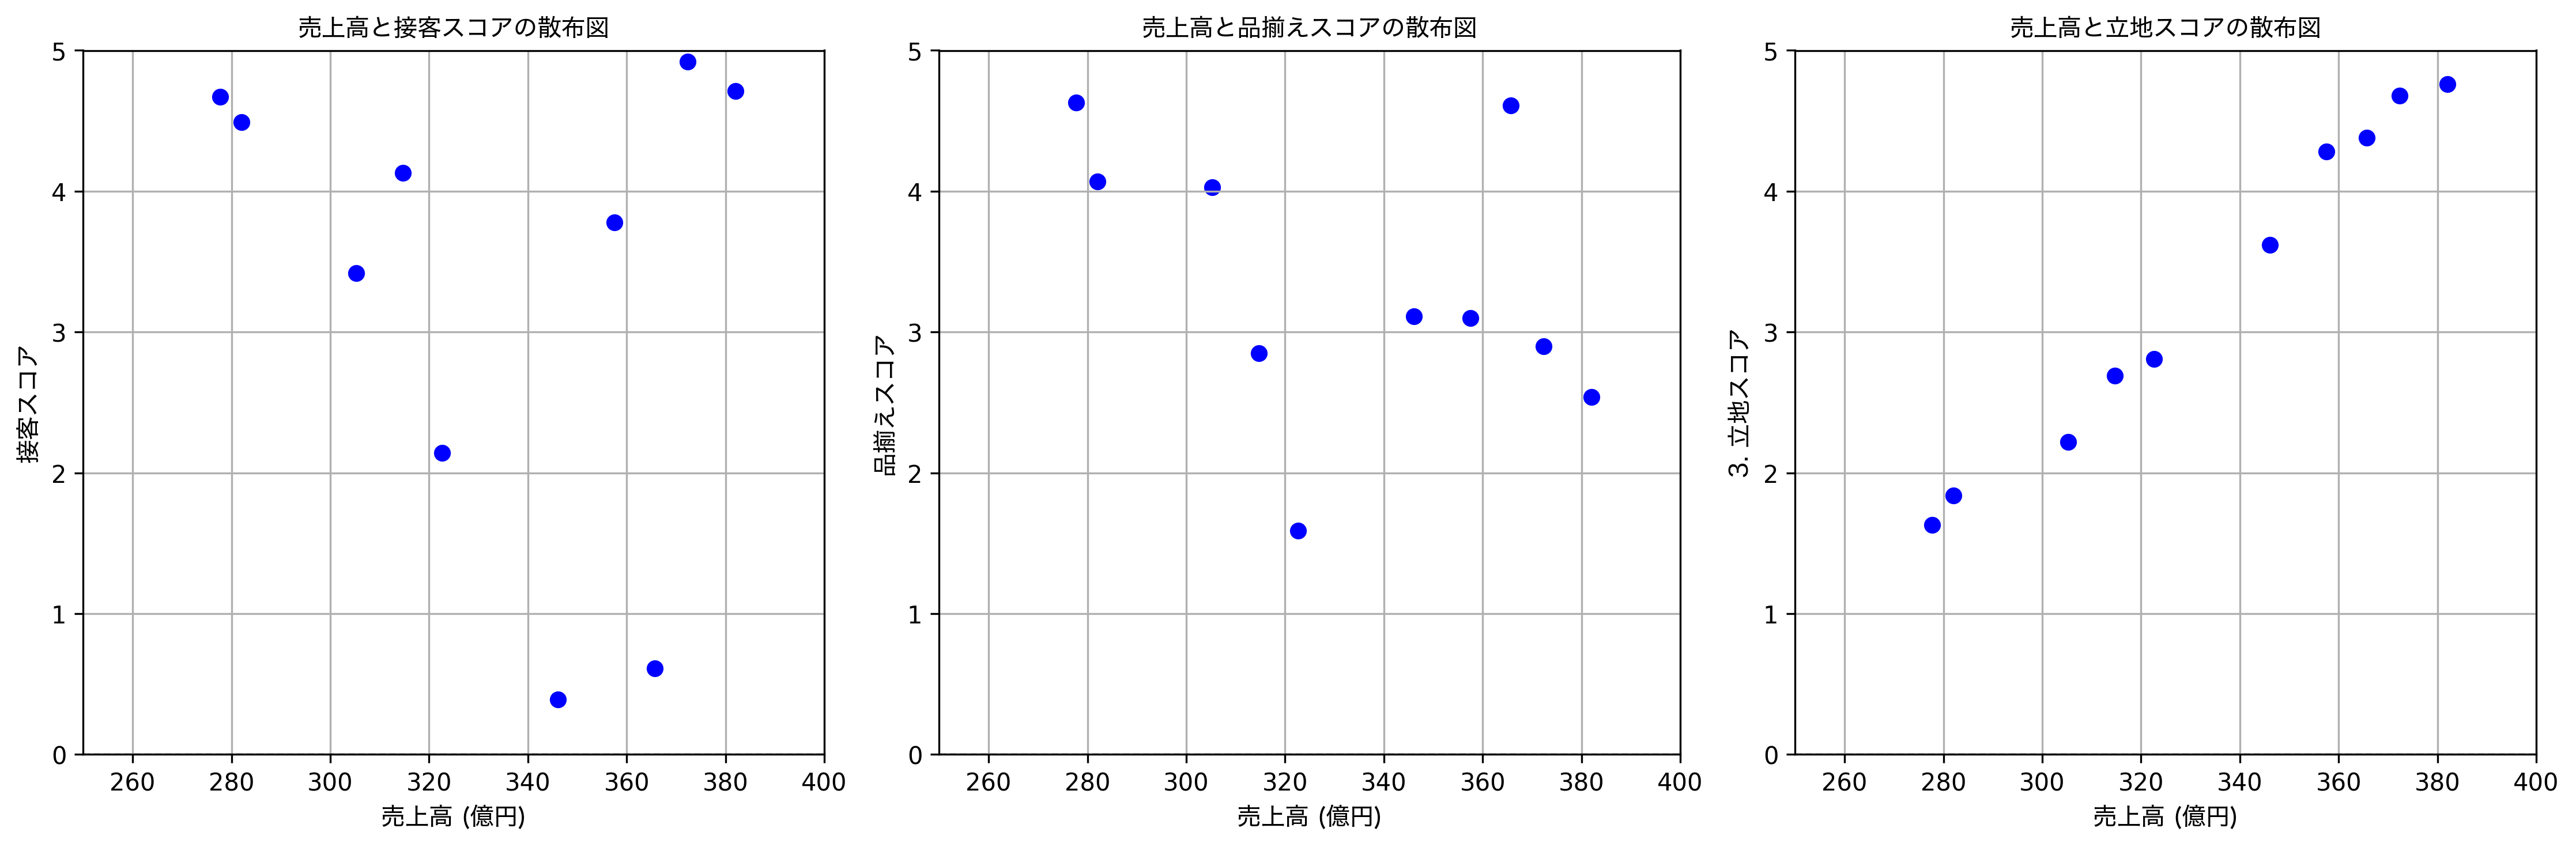
\includegraphics[width=1\textwidth]{graph/g.png}
    \caption{売上高と各項目の相関}
    \label{fig:correlation}
\end{figure}


\end{document}



























